%File: formatting-instruction.tex
\documentclass[letterpaper]{article}
\usepackage{aaai}
\usepackage{times}
\usepackage{helvet}
\usepackage{courier}
\usepackage{graphicx}
\usepackage{fontenc}
\frenchspacing
\setlength{\pdfpagewidth}{8.5in}
\setlength{\pdfpageheight}{11in}
\pdfinfo{
/Title (Insert Your Title Here)
/Author (Put All Here, Separated by Commas)}
\setcounter{secnumdepth}{0}  
 \begin{document}
% The file aaai.sty is the style file for AAAI Press 
% proceedings, working notes, and technical reports.
%
\title{Proyecto Semestral 2: \\Algoritmos de Machine Learning {}}
\author{Farinango Yadira; Rodriguez Genith\\
}
\maketitle
\begin{abstract}
\begin{quote}
Este artículo explora e identifica el uso de dos algoritmos de aprendizaje diferentes (Logistic Regression, Decision Tree Classifier), para clasificar el ancho y largo de los petalos de la flores de una base de datos llamada IRIS.cvs. Tambien se va apresentar un análisis comparativo de los algoritmos y se mostrará cual de los dos métodos aplicados sera mas eficiente.
\end{quote}
\end{abstract}

\section{INTRODUCCIÒN}
Los algoritmos de clasificación como Logistic Regression y Decision Tree Classifier se utilizan actualmente como una variación de conjunto de datos con los cuales se pueden mostrar un buen o un mal resultado al momento de clasificarlos.
En este artìculo, los dos algoritmos mensionados anteriormente se proponen como mètodos de filtrado para contabilizar los petalos y para comprobar su rendimiento. Dentro de cada algoritmo, se va a desarrollar un ajuste de parametros para mejorar los resultados previstos y posibles en el uso del mètodo de busqueda en cuadrìcula.

En cuanto al conjunto de los datos esta dividido en conjuntos de entrenamiento y prueba. La forma en la que dividimos los datos fueron mediante las especies de las flores (setosa, virginica, versicolor). En lo cual se puedo optener un buen enfoque para difrenciar las carcteristicas de los petalos. Luego se entreno cada uno de los dos algoritmos usando el conjunto de entrenamiento, y en cuanto al ultimo paso, procedimos a evaluar sus desempeños en la matrìz de prueba.

Por el bien el algoritmo de clasificación, los conjuntos entrenados y prueba tenian que expresarse como un vector. Las dimensiones que se obtuvo en el vector corresponden a la frecuencia de lo ancho y largo de los petalos. La matríz de resultados para los dos algoritmo muestra una comparacion de satisfacción o asi mismo muestra el la caida de uno de los dos argoritmos.

\section{MARCO TEÒRICO}
\subsection{Machine Learning}
Machine Learning o aprendizaje automático es un campo científico y particularmente una subcategoria de inteligencia artificial, en el cual consiste en dejar que los algoritmos descubran los patrones recurrentes, en conjunto de datos esto puede ser por nùmeros, palabras, imágenes y estadisticas.
Todo lo que se pueda almacenar digitalmente puede servir como un dato para el machine learning. Al detectar patrones en esos datos, los algoritmos aprenden y mejoran su rendimiento en la ejecucuiòn de una tarea especìfica.

\section{ALGORITMOS EMPLEADOS}
\begin{enumerate}
\item 
\textbf{Logistic Regression}  
\\La regresión logística es un método estadístico que trata de modelar la probabilidad de una variable cualitativa binaria (dos posibles valores) en función de una o más variables independientes. La principal aplicación de la regresión logística es la creación de modelos de clasificación binaria.

Se llama regresión logística simple cuando solo hay una variable independiente y regresión logística múltiple cuando hay más de una. Dependiendo del contexto, a la variable modelada se le conoce como variable dependiente o variable respuesta, y a las variables independientes como regresores, predictores o features.

A lo largo de este documento, se describen de forma progresiva los fundamentos teóricos de la regresión logística, los principales aspectos prácticos a tener en cuenta y ejemplos de cómo crear este tipo de modelos en Python.
\begin{itemize}
    \item 
    \textbf{Clasificador de Logistic Regression}
    \\Dado un conjunto de entradas en X y Y, se difinen los parametros tanto para entrenamiento como para evaluación, mediante la cración del modelo de clasificación se puede difinir una entrada y salida mediante un objeto en la fase de entrenamiento en la cual se pone en forma al modelo para que se pueda encontrar una salida y una entrada, con la ayuda de la predicción empirica se obtendra una predicción de 1 a 0 para poder fundamentar en entrenamiento mediante una matriz de evaluación conocida como métrica de confución que se encarga de mostrar y clasificar los valores de satisfacción mediante un reporte general tanto del valor real como del valor de la predicción, y asi lograr obtener la precisión del modelo y la exactitud del mismo.  
\end{itemize}
\item 
\textbf{Decision Tree} 
\\Un árbol de decisión es un algoritmo de aprendizaje supervisado no paramétrico, que se utiliza tanto para tareas de clasificación como de regresión. Tiene una estructura de árbol jerárquica, que consta de un nodo raíz, ramas, nodos internos y nodos hoja.

Un árbol de decisión comienza con un nodo raíz, que no tiene ramas entrantes. Las ramas salientes del nodo raíz alimentan los nodos internos, también conocidos como nodos de decisión. En función de las características disponibles, ambos tipos de nodos realizan evaluaciones para formar subconjuntos homogéneos, que se indican mediante nodos hoja o nodos terminales. Los nodos hoja representan todos los resultados posibles dentro del conjunto de datos.
\begin{itemize}
    \item 
    \textbf{Clasificador de Decision Tree}
    \\Dado un conjunto de entradas en X y Y, se difinen los parametros tanto para entrenamiento como para evaluación, mediante el arbol de decisión que consiste en clasificar correctamente la variedad de la flor iris a partir del ancho y largo de los pétalos y sépalos.
    
    Se manda a llamr al modelo para que clasifique los valores de la entrada y salida del objeto con el fin de entrenar el modelo mediante la predicción que esta generara la posibilidad de que ocurra la clasificación mediante el entrenamiento de la matriz se comprobara si esta cumple con la clasificación de los pétalos mediante la métrica de confución se generar el valor de satisfacción mediante la clasificación de las  setosa, versicolor y virginica, se prodra verificar mediante un reporte el valor real que tendran para asi lograr general el modelo con exactitud. 
\end{itemize}
\end{enumerate}

\section{RESULTADO}
En esta sección, se muestra un conjunto de datos que contiene 50 muestras de cada una de tres especies de Iris: Iris setosa, Iris virginica e Iris versicolor, para cada una de estas especies se midieron cuatro rasgos de cada muestra: la longitud y el ancho del sépalos y pétalos.

\begin{figure}[h]
    \centering
    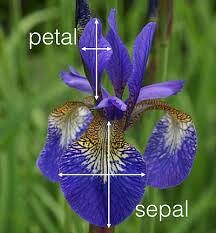
\includegraphics[width=5cm]{IRIS.jpg}
    \caption{Ancho y largo de la flor}
\end{figure}

En primer lugar se tuvo que importar las librerías numpy y pandas, y asi misma se prosigui a extraer los datos de la base de datos IRIS.csv, y se mando a visualizar un total de 5 datos mediante la instrucción head. Se pudo observar donde están las características tanto de ancho y longitud del sépalo y pétalo, y a su vez el nombre de cada una de las especies posteriormente se pudo procesar el analizar los datos mediante las columnas ya que estas contienen 150 datos, en las primeras tenemos datos flotantes mientras que la última contiene datos objetivos y es justamente acá en donde se encuentra la información de las especies de la flor.

Por último, verificamos la distribución de los datos de acuerdo a las especies de Iris, para ello utilizamos la instrucción groupby, especificando la columna Species y el tamaño de la misma. Se pudo observar que se tenia 50 datos para cada una de las especies, Iris setosa, Iris versicolor e Iris Virginica. Con esto se pudo demostar mediante la libreria matplotlib la visualización de los datos mediante graficas.

\begin{figure}[h]
    \centering
    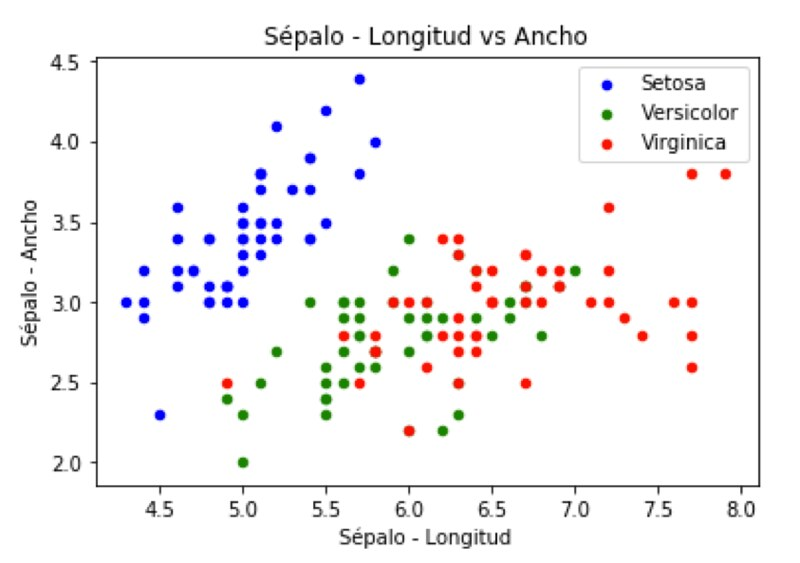
\includegraphics[width=5cm]{sepalo.jpg}
    \caption{Clasificación del tipo de flores}
\end{figure}

 Como respuesta a la investigación se evaluarón los efectos de los dos algoritmos de clasificación (Logistic Regression y Decision Tree), en función de diferentes hiperparámetros y también de diferentes tamaños de características para encontrar el modelo óptimo para el filtrado del ancho y largo de los pétalos y sépalos. Posteriormente, el rendimiento del filtrado se mide en términos de precisión. Significa que cada una de las clasificaciones se evaluarón utilizando una puntuación de precisión modificada en el modelo con el fin de obtener un modelo que cumpla con una exactitud muy buena en el desarrollo del modelo utilizando la función de matriz de confusión para calcular la exactitud de los modelos de algoritmos.

\section{RECOMENDACIÓN}
 Después de emplear los dos algoritmos de clasificación mediante la experimentación hicimos pruebas en cada uno de
los modelos. No podemos decir cuál debe seleccionarse, pero está
claro que hasta ahora el clasificador de Decision Tree se desempeñó bien en comparación con el clasificador Logistic Regression. Para tomar la decisión final, se evalúo mediante la evaluacioón en metrica para conoser la satisfacción así poder clasificar las flores mediante la metrica confusión.

Para elegir el modelo óptimo, tenemos que mirar
cuidadosamente el reporte general entre los valores reales y la predicción para conoser la precisión tanto del pétalo y sépalo para que se pueda generar un modelo que cumpla con la exactitud que contiene los algoritmos. Y finalmente salimos
con la solución de que la Decision Tree es la que cumple
con los requisitos.

\section{CONCLUSIONES}
En este artículo, proponemos dos métodos de aprendizaje automático para el filtrado de los pétalos y sépalos de flores y presentamos una evaluación empírica de ellos en un conjunto de datos que se nos ha proporcionado. Estos enfoques incluyen el clasificador Logistic Regression, el clasificador Decision Tree. El experimento llevado a cabo para probar el rendimiento de estos algoritmos es para encontrar valores óptimos de los hiperparámetros con el uso de un optimizador utilizando la matriz confunsión. Los resultados experimentales muestran que el clasificador Decision Tree es más optimo de los algoritmos utilizados ya que ofrece una exactitud mayor al clasificardor Logistic Regression. Por lo tanto,
seleccionamos el clasificador de Decision Tree como el filtrado final de la clasificación de los valores reales. También elegimos este porque muestra una precisión y exactitud acorde al modelo del algoritmo y determinar un modelo eficiente. 

\section{BIBLIOGRAFIAS}
\smallskip \noindent \textit{Sitio Web}\\
Ligdi Gonzalez,  agosto 31, 2018. \textit{Aprende IA.} Recuperado de: https://aprendeia.com/machine-learning-clasificador-flor-iris-python/

\smallskip \noindent \textit{Página Web}\\
Robinson Castro, España, mayo 26, 2015. \textit{IBM} Recuperado de: https://www.ibm.com/es-es/topics/decision-trees

\smallskip \noindent \textit{Página Web}\\
Joaquín Rodrigo, Noviembre 13, 2020. \textit{Cienciadedatos.net} Recuperado de: https://www.cienciadedatos.net/documentos/py17-regresion-logistica-python.html

\smallskip \noindent \textit{Sitio Web}\\
Rebeca Bentata, diciembre 13, 2021. \textit{DataScientest} Recuperado de: https://datascientest.com/es/machine-learning-definicion-funcionamiento-usos

\end{document}